\iffalse 
\documentclass[SoftwareDesign/SoftwareDesign_main.tex]{subfiles}
\fi

\documentclass{article}

\begin{document}
\section{Design av Edit User page}
Dette avsnittet presenterer designet av Viewet og den tilhørende ViewModelen til EditUserPage. Den er designet med ViewFirst prinsippet på samme måte som HeaderBar.
\subsection{Design av View til Edit User Page}
Edit user page skal på mange måter fungere på samme måte som CarProfile. Den skal være siden som brukeren kan navigere til for å redigere bruker informasjonen som er lagret om dem i CarnGo.

\begin{figure}[H]
    \centering
    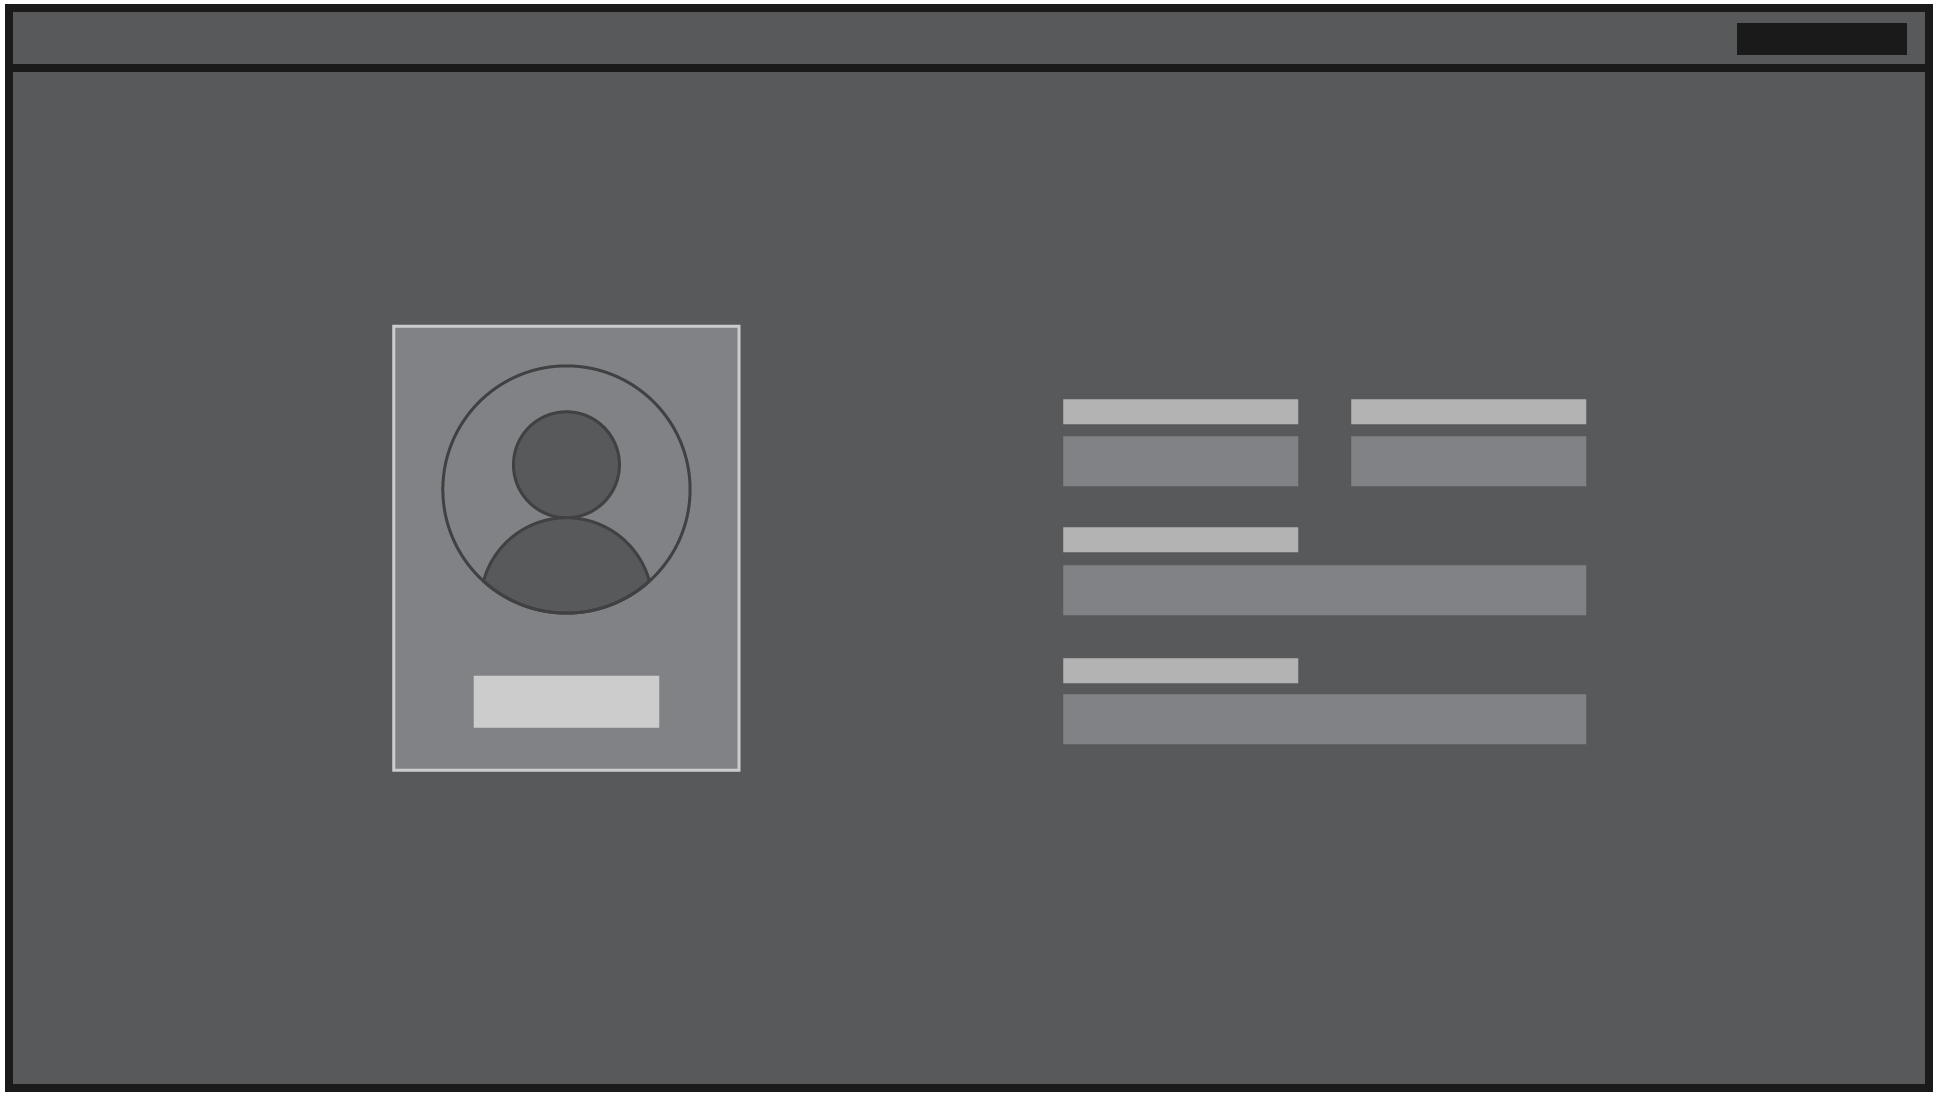
\includegraphics[width=\textwidth]{SoftwareDesign/MVVMDesigns/Graphics/EditUserPage.png}
    \caption{Edit User WireFrame}
    \label{fig:EditUserWireFrame}
\end{figure}


\subsection{Design av ViewModel til EditUser}
ViewModellen skal lagre en kopi av UserModelen som den skal utføre alle endringene på frem til brukeren trykke på save knappen. Når det trykkes på save skal den kopiere dataen over i brukerens UserModel og lagre endringene på databasen.

\end{document}